\documentclass[12pt,letterpaper]{article}
\usepackage{graphicx,textcomp}
\usepackage{natbib}
\usepackage{setspace}
\usepackage{fullpage}
\usepackage{color}
\usepackage[reqno]{amsmath}
\usepackage{amsthm}
\usepackage{fancyvrb}
\usepackage{amssymb,enumerate}
\usepackage[all]{xy}
\usepackage{endnotes}
\usepackage{lscape}
\newtheorem{com}{Comment}
\usepackage{float}
\usepackage{hyperref}
\newtheorem{lem} {Lemma}
\newtheorem{prop}{Proposition}
\newtheorem{thm}{Theorem}
\newtheorem{defn}{Definition}
\newtheorem{cor}{Corollary}
\newtheorem{obs}{Observation}
\usepackage[compact]{titlesec}
\usepackage{dcolumn}
\usepackage{tikz}
\usetikzlibrary{arrows}
\usepackage{multirow}
\usepackage{xcolor}
\newcolumntype{.}{D{.}{.}{-1}}
\newcolumntype{d}[1]{D{.}{.}{#1}}
\definecolor{light-gray}{gray}{0.65}
\usepackage{url}
\usepackage{listings}
\usepackage{color}

\definecolor{codegreen}{rgb}{0,0.6,0}
\definecolor{codegray}{rgb}{0.5,0.5,0.5}
\definecolor{codepurple}{rgb}{0.58,0,0.82}
\definecolor{backcolour}{rgb}{0.95,0.95,0.92}

\lstdefinestyle{mystyle}{
	backgroundcolor=\color{backcolour},   
	commentstyle=\color{codegreen},
	keywordstyle=\color{magenta},
	numberstyle=\tiny\color{codegray},
	stringstyle=\color{codepurple},
	basicstyle=\footnotesize,
	breakatwhitespace=false,         
	breaklines=true,                 
	captionpos=b,                    
	keepspaces=true,                 
	numbers=left,                    
	numbersep=5pt,                  
	showspaces=false,                
	showstringspaces=false,
	showtabs=false,                  
	tabsize=2
}
\lstset{style=mystyle}
\newcommand{\Sref}[1]{Section~\ref{#1}}
\newtheorem{hyp}{Hypothesis}

\title{Problem Set 3}
\date{Due: November 19, 2022}
\author{Applied Stats/Quant Methods 1}


\begin{document}
	\maketitle
	\section*{Instructions}
	\begin{itemize}
		\item Please show your work! You may lose points by simply writing in the answer. If the problem requires you to execute commands in \texttt{R}, please include the code you used to get your answers. Please also include the \texttt{.R} file that contains your code. If you are not sure if work needs to be shown for a particular problem, please ask.
	\item Your homework should be submitted electronically on GitHub.
	\item This problem set is due before 23:59 on Sunday November 19, 2023. No late assignments will be accepted.

	\end{itemize}

		\vspace{.25cm}
	
\noindent In this problem set, you will run several regressions and create an add variable plot (see the lecture slides) in \texttt{R} using the \texttt{incumbents\_subset.csv} dataset. Include all of your code.

	\vspace{.5cm}
\section*{Question 1}
\vspace{.25cm}
\noindent We are interested in knowing how the difference in campaign spending between incumbent and challenger affects the incumbent's vote share. 
	\begin{enumerate}
		\item Run a regression where the outcome variable is \texttt{voteshare} and the explanatory variable is \texttt{difflog}.	
	\lstinputlisting[language=R, firstline=34, lastline=38]{PS3.R}  
\begin{verbatim}
Call:lm(formula = voteshare ~ difflog, data = inc.sub)
Residuals:     Min       1Q   Median       3Q      Max 
-0.26832 -0.05345 -0.00377  0.04780  0.32749 
Coefficients:            Estimate Std. Error t value Pr(>|t|)  
  (Intercept) 0.579031   0.002251  257.19   <2e-16 ***
  difflog     0.041666   0.000968   43.04   <2e-16 ***
  ---
  Signif. codes:  0 ‘***’ 0.001 ‘**’ 0.01 ‘*’ 0.05 ‘.’ 0.1 ‘ ’ 1
  Residual standard error: 0.07867 on 3191 degrees of freedom
  Multiple R-squared:  0.3673,	Adjusted R-squared:  0.3671 
  F-statistic:  1853 on 1 and 3191 DF,  p-value: < 2.2e-16
\end{verbatim} 	
		\item Make a scatterplot of the two variables and add the regression line. 	
\lstinputlisting[language=R, firstline=39, lastline=44]{PS3.R} 
	\begin{figure}[h!]\centering
		\caption{\footnotesize scatter plot with line.}
		\label{fig:plot_1}
		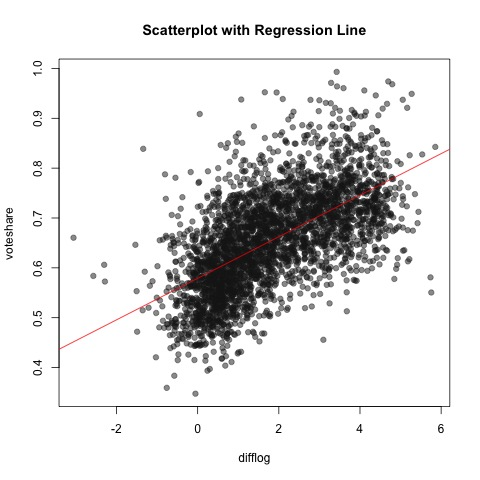
\includegraphics[width=.45\textwidth]{voteshare_difflog.jpeg}
	\end{figure}

		\item Save the residuals of the model in a separate object.	
	\lstinputlisting[language=R, firstline=45, lastline=45]{PS3.R} 	
		\item Write the prediction equation.\vspace{1cm}
voteshare=intercept+slope ×difflog
\lstinputlisting[language=R, firstline=46, lastline=50]{PS3.R} 	
voteshare = 0.579030710920674 + 0.0416663238227399 * difflog 
	\end{enumerate}
	
\newpage

\section*{Question 2}
\noindent We are interested in knowing how the difference between incumbent and challenger's spending and the vote share of the presidential candidate of the incumbent's party are related.	\vspace{.25cm}
	\begin{enumerate}
		\item Run a regression where the outcome variable is \texttt{presvote} and the explanatory variable is \texttt{difflog}.
\lstinputlisting[language=R, firstline=51, lastline=53]{PS3.R} 	
\begin{verbatim}
Call:lm(formula = presvote ~ difflog, data = inc.sub)
Residuals:     Min       1Q   Median       3Q      Max 
-0.32196 -0.07407 -0.00102  0.07151  0.42743 
Coefficients:            
							Estimate Std. Error t value Pr(>|t|)    
(Intercept) 0.507583   0.003161  160.60   <2e-16 ***
difflog     0.023837   0.001359   17.54   <2e-16 ***
---
Signif. codes:  0 ‘***’ 0.001 ‘**’ 0.01 ‘*’ 0.05 ‘.’ 0.1 ‘ ’ 1
Residual standard error: 0.1104 on 3191 degrees of freedom
Multiple R-squared:  0.08795,	Adjusted R-squared:  0.08767 
F-statistic: 307.7 on 1 and 3191 DF,  p-value: < 2.2e-16
\end{verbatim} 	
		\item Make a scatterplot of the two variables and add the regression line. 
\lstinputlisting[language=R, firstline=54, lastline=58]{PS3.R} 	\vspace{7cm}
	\begin{figure}[h!]\centering
		\caption{\footnotesize scatter plot presvote and difflog.}
		\label{fig:plot_2}
		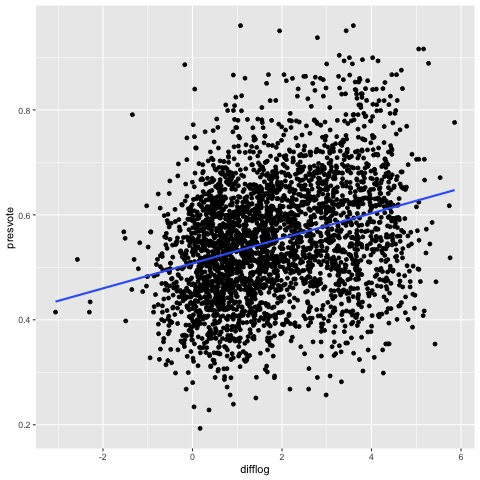
\includegraphics[width=.75\textwidth]{presvote_difflog.jpeg}
	\end{figure}

		\item Save the residuals of the model in a separate object.	
\lstinputlisting[language=R, firstline=59, lastline=59]{PS3.R} 	
		\item Write the prediction equation.
\lstinputlisting[language=R, firstline=60, lastline=63]{PS3.R} 	
"presvote = 0.507583328405015 + 0.023837233841334 * difflog "
	\end{enumerate}
	
	\newpage	
\section*{Question 3}

\noindent We are interested in knowing how the vote share of the presidential candidate of the incumbent's party is associated with the incumbent's electoral success.
	\vspace{.25cm}
	\begin{enumerate}
		\item Run a regression where the outcome variable is \texttt{voteshare} and the explanatory variable is \texttt{presvote}.
\lstinputlisting[language=R, firstline=64, lastline=66]{PS3.R} 	
\begin{verbatim}
Call:lm(formula = voteshare ~ presvote, data = inc.sub)
Residuals:     Min       1Q   Median       3Q      Max 
-0.27330 -0.05888  0.00394  0.06148  0.41365 
Coefficients:            Estimate Std. Error t value Pr(>|t|)    
(Intercept) 0.441330   0.007599   58.08   <2e-16 ***
presvote    0.388018   0.013493   28.76   <2e-16 ***
---
Signif. codes:  0 ‘***’ 0.001 ‘**’ 0.01 ‘*’ 0.05 ‘.’ 0.1 ‘ ’ 1
Residual standard error: 0.08815 on 3191 degrees of freedom
Multiple R-squared:  0.2058,	Adjusted R-squared:  0.2056 
F-statistic:   827 on 1 and 3191 DF,  p-value: < 2.2e-16
\end{verbatim} 	
			\vspace{3cm}
		\item Make a scatterplot of the two variables and add the regression line. 
\lstinputlisting[language=R, firstline=68, lastline=72]{PS3.R} 	

	\begin{figure}[h!]\centering
		\caption{\footnotesize scatter plot presvote and voteshare.}
		\label{fig:plot_3}
		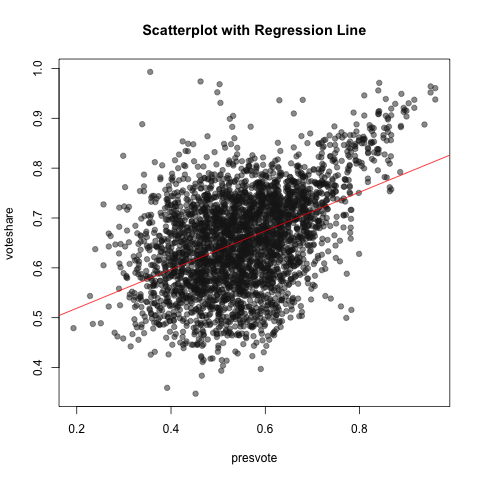
\includegraphics[width=.65\textwidth]{scatterplot_voteshare_presvote.png}
	\end{figure}

			\vspace{5cm}
		\item Write the prediction equation.
\lstinputlisting[language=R, firstline=74, lastline=79]{PS3.R} 	
"voteshare = 0.441329881204298 + 0.38801844338744 * presvote"
	\end{enumerate}
	

\newpage	
\section*{Question 4}
\noindent The residuals from part (a) tell us how much of the variation in \texttt{voteshare} is $not$ explained by the difference in spending between incumbent and challenger. The residuals in part (b) tell us how much of the variation in \texttt{presvote} is $not$ explained by the difference in spending between incumbent and challenger in the district.
	\begin{enumerate}
		\item Run a regression where the outcome variable is the residuals from Question 1 and the explanatory variable is the residuals from Question 2.
\lstinputlisting[language=R, firstline=80, lastline=83]{PS3.R} 	
\begin{verbatim}
Call:lm(formula = residuals_voteshare ~ residuals_presvote, data = inc.sub)
Residuals:     Min       1Q   Median       3Q      Max 
-0.25928 -0.04737 -0.00121  0.04618  0.33126 
Coefficients:                     
                      			Estimate Std. Error t value Pr(>|t|)    
(Intercept)       
 											-1.942e-18  1.299e-03    0.00   1    
 residuals_presvote  2.569e-01  1.176e-02   21.84   <2e-16 ***
 ---
 Signif. codes:  0 ‘***’ 0.001 ‘**’ 0.01 ‘*’ 0.05 ‘.’ 0.1 ‘ ’ 1
 Residual standard error: 0.07338 on 3191 degrees of freedom
 Multiple R-squared:   0.13,	Adjusted R-squared:  0.1298 
 F-statistic:   477 on 1 and 3191 DF,  p-value: < 2.2e-16
\end{verbatim} 	
		\item Make a scatterplot of the two residuals and add the regression line. 	
\lstinputlisting[language=R, firstline=87, lastline=91]{PS3.R} 	
	\begin{figure}[h!]\centering
	\caption{\footnotesize scatterplot two residuals.}
	\label{fig:plot_4}
	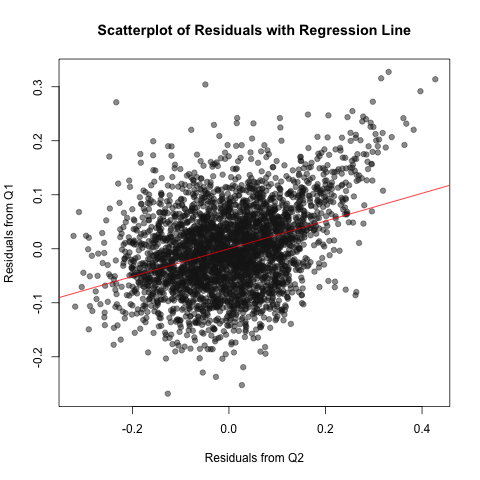
\includegraphics[width=.65\textwidth]{scatterplot_residuals_q1_q2.png}
\end{figure}	
\vspace{5cm}
		\item Write the prediction equation.
\lstinputlisting[language=R, firstline=93, lastline=98]{PS3.R} 
\begin{verbatim}
"Residuals_Q1(voteshare) = -1.94153862344556e-18 + 
0.256877012700097 * Residuals_Q2 (presvote)"
\end{verbatim} 	
	\end{enumerate}
	
	\newpage	

\section*{Question 5}
\noindent What if the incumbent's vote share is affected by both the president's popularity and the difference in spending between incumbent and challenger? 
	\begin{enumerate}
		\item Run a regression where the outcome variable is the incumbent's \texttt{voteshare} and the explanatory variables are \texttt{difflog} and \texttt{presvote}.	
\lstinputlisting[language=R, firstline=99, lastline=102]{PS3.R} 
\begin{verbatim}	
Call:lm(formula = voteshare ~ difflog + presvote, data = inc.sub)
Residuals:     Min       1Q   Median       3Q      Max 
-0.25928 -0.04737 -0.00121  0.04618  0.33126 
Coefficients:             Estimate Std. Error t value Pr(>|t|)    
(Intercept) 0.4486442  0.0063297   70.88   <2e-16 ***
difflog     0.0355431  0.0009455   37.59   <2e-16 ***
presvote    0.2568770  0.0117637   21.84   <2e-16 ***
---Signif. codes: 
 0 ‘***’ 0.001 ‘**’ 0.01 ‘*’ 0.05 ‘.’ 0.1 ‘ ’ 1
 Residual standard error: 0.07339 on 3190 degrees of freedom
 Multiple R-squared:  0.4496,	Adjusted R-squared:  0.4493 
 F-statistic:  1303 on 2 and 3190 DF,  p-value: < 2.2e-16
\end{verbatim} 	
		\item Write the prediction equation.
\lstinputlisting[language=R, firstline=103, lastline=109]{PS3.R} 	
"voteshare = 0.448644221823622 + 0.0355430864025444 * difflog + 0.256877012700098 * presvote" \vspace{6cm}
		\item What is it in this output that is identical to the output in Question 4? Why do you think this is the case?
		
		\end{enumerate}
the coefficient for presvote is in question 5 is same as the coefficient for residuals(presvote) in the model with residuals in q4. To interpret, this coefficient in q4 context tells us with one unit increase  in the  residuals from presvore-difflog regression, which is the variation not explained by difference in spending (difflog) with regard to presvote, there is about on average 0.26 unit increase in the residuals from votshare-difflog regression model, which is variation not explained by difflog with regard to voteshare. In other words, if we remove the effect of difflog (holding it constant), one unit increase in the presvote will increase  0.26 unit of voteshare on average, which is also what the coeeficient for presvote in question 5 tells us. To illustrate the point, we can also see a side by side comparison between the added variable plot of presvote to voteshare conditioned on difflog and the scatter plot of residuals and conclude they are showing the same thing. Based on this observation and since the pvalue is very small so it's significant, we can conclude that presvote is a variable that can explain certain variation in voteshare in addition to difflog, so we should probably keep it in our model so as to not commit omitted variable bias. Hence we found evidence that support the incumbent's vote share is affected by both the president's popularity and the difference in spending between incumbent and challenger.

\begin{figure}
	\begin{minipage}[t]{0.5\textwidth} 
		\centering
		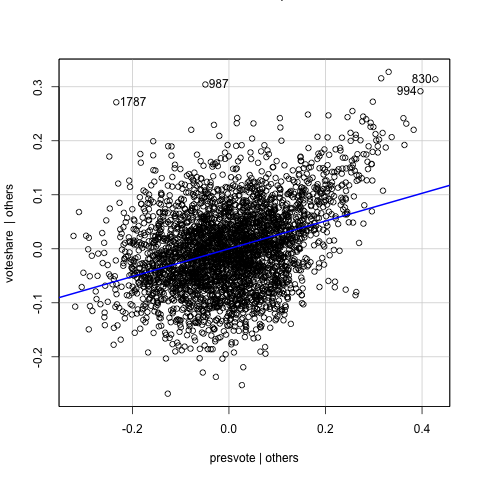
\includegraphics[width=\linewidth]{added_variable_plot_presvote.png}
		\caption{added variable plot}
		\label{fig:subfig1}
	\end{minipage}%
	\begin{minipage}[t]{0.5\textwidth} 
		\centering
		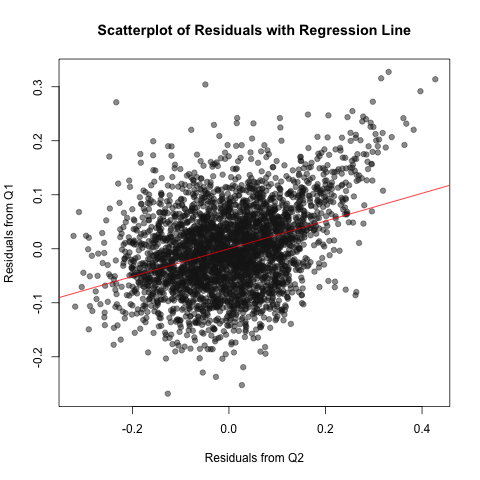
\includegraphics[width=\linewidth]{scatterplot_residuals_q1_q2.png}
		\caption{residuals scatterplot}
		\label{fig:subfig2}
	\end{minipage}
	\caption{comparison}
	\label{fig:combined}
\end{figure}






\end{document}
